\documentclass[12pt, titlepage]{article}

\usepackage{fullpage}
\usepackage[round]{natbib}
\usepackage{multirow}
\usepackage{booktabs}
\usepackage{tabularx}
\usepackage{graphicx}
\usepackage{float}
\usepackage{hyperref}
\usepackage{pdfpages}
\usepackage{pdflscape}

\hypersetup{
    colorlinks,
    citecolor=black,
    filecolor=black,
    linkcolor=red,
    urlcolor=blue
}
\usepackage[round]{natbib}
\usepackage{multirow}

\input{../Comments}
%% Common Parts

\newcommand{\progname}{Measuring Microstructure Changes During Thermal Treatment} % PUT YOUR PROGRAM NAME HERE
\newcommand{\authname}{Team \#30, ReSprint
\\ Edwin Do
\\ Joseph Braun
\\ Timothy Chen
\\ Abdul Nour Seddiki
\\ Tyler Magarelli
} % AUTHOR NAMES                  

\usepackage{hyperref}
    \hypersetup{colorlinks=true, linkcolor=blue, citecolor=blue, filecolor=blue,
                urlcolor=blue, unicode=false}
    \urlstyle{same}
                                


\begin{document}

\title{Verification and Validation Report: \progname} 
\author{\authname}
\date{\today}
	
\maketitle

\pagenumbering{roman}

\section{Revision History}


\begin{tabularx}{\textwidth}{p{3cm}p{3cm}X}
\toprule {\bf Date} & {\bf Developer} & {\bf Change}\\
\midrule
Mar 8 2023 & Edwin Do & Added usability test results \\
Mar 8 2023 & Edwin Do & Added Traceability matrices \\
Mar 8, 2023 & Joseph Braun & Added Sections 5, 7, 8 \\
Mar 8, 2023 & Joseph Braun & Added Reflection \\
\bottomrule
\end{tabularx}

~\newpage

\section{Symbols, Abbreviations and Acronyms}
change capacity to size

\renewcommand{\arraystretch}{1.2}
\begin{tabular}{l l} 
  \toprule		
  \textbf{symbol} & \textbf{description}\\
  \midrule 
  T & Test\\
  \bottomrule
\end{tabular}\\

\wss{symbols, abbreviations or acronyms -- you can reference the SRS tables if needed}

\newpage

\tableofcontents

\listoftables %if appropriate

\listoffigures %if appropriate

\newpage

\pagenumbering{arabic}

This document ...
Section 11 Code Coverage Metrics is removed.

\section{Functional Requirements Evaluation}

\section{Nonfunctional Requirements Evaluation}

In the section

\pagebreak
\subsection{Usability}
The table below shows the results of our usability tests based on the tests in the V\&V plan based on the requirements mentioned in the SRS.
Each requirement can be traced to multiple unit tests and the usability survey used can be found in the Appendix.\\
\\
\begin{tabular}{ |p{2.5cm}||p{2cm}|p{4cm}|p{4cm}|p{1.5cm}| }
  \hline
  \multicolumn{5}{|c|}{Usability Tests} \\
  \hline
  Test Requirement & Related Unit Tests & Description & Expected Result & Result\\
  \hline
  NF-UT1   & AF  & Completing tasks without additional assistance. & User will be complete tasks successfully & PASS\\
  \hline
  NF-UT2   & AX  & Interact with interace to modify parameters. & User will be able to modify the parameters accurately and quickly.& PASS\\
  \hline
  NF-UT3   & AL  & Completing all tasks with limited number of mistakes & User will be able to complete all tasks with \textsl{MAX\_MISTAKE} & PASS\\
  \hline
  NF-UT3   & AL  & Verifying if interacting with the application previously improves ease of use (learnability)  & User will be able to complete the tasks more quickly and accurately the second time & PASS\\
  \hline
  NF-UT5   & AS  & Verifying how calculations are performed is hidden &  User will not know how calculations are performed after doing the set of tasks & PASS\\
  \hline
  NF-UT6   & AS  & Verifying appropriate application size upon installation&  User will install application onto computer and verify that the application size is less than or equal to \textsl{MAX\_SIZE} & PASS\\
  \hline
 \end{tabular}
		
\subsection{Performance}

\subsection{etc.}
	

\section{Comparison to Existing Implementation}	

\noindent Below is an image of the exisiting implementation's GUI.

\begin{figure}[H]
\centerline{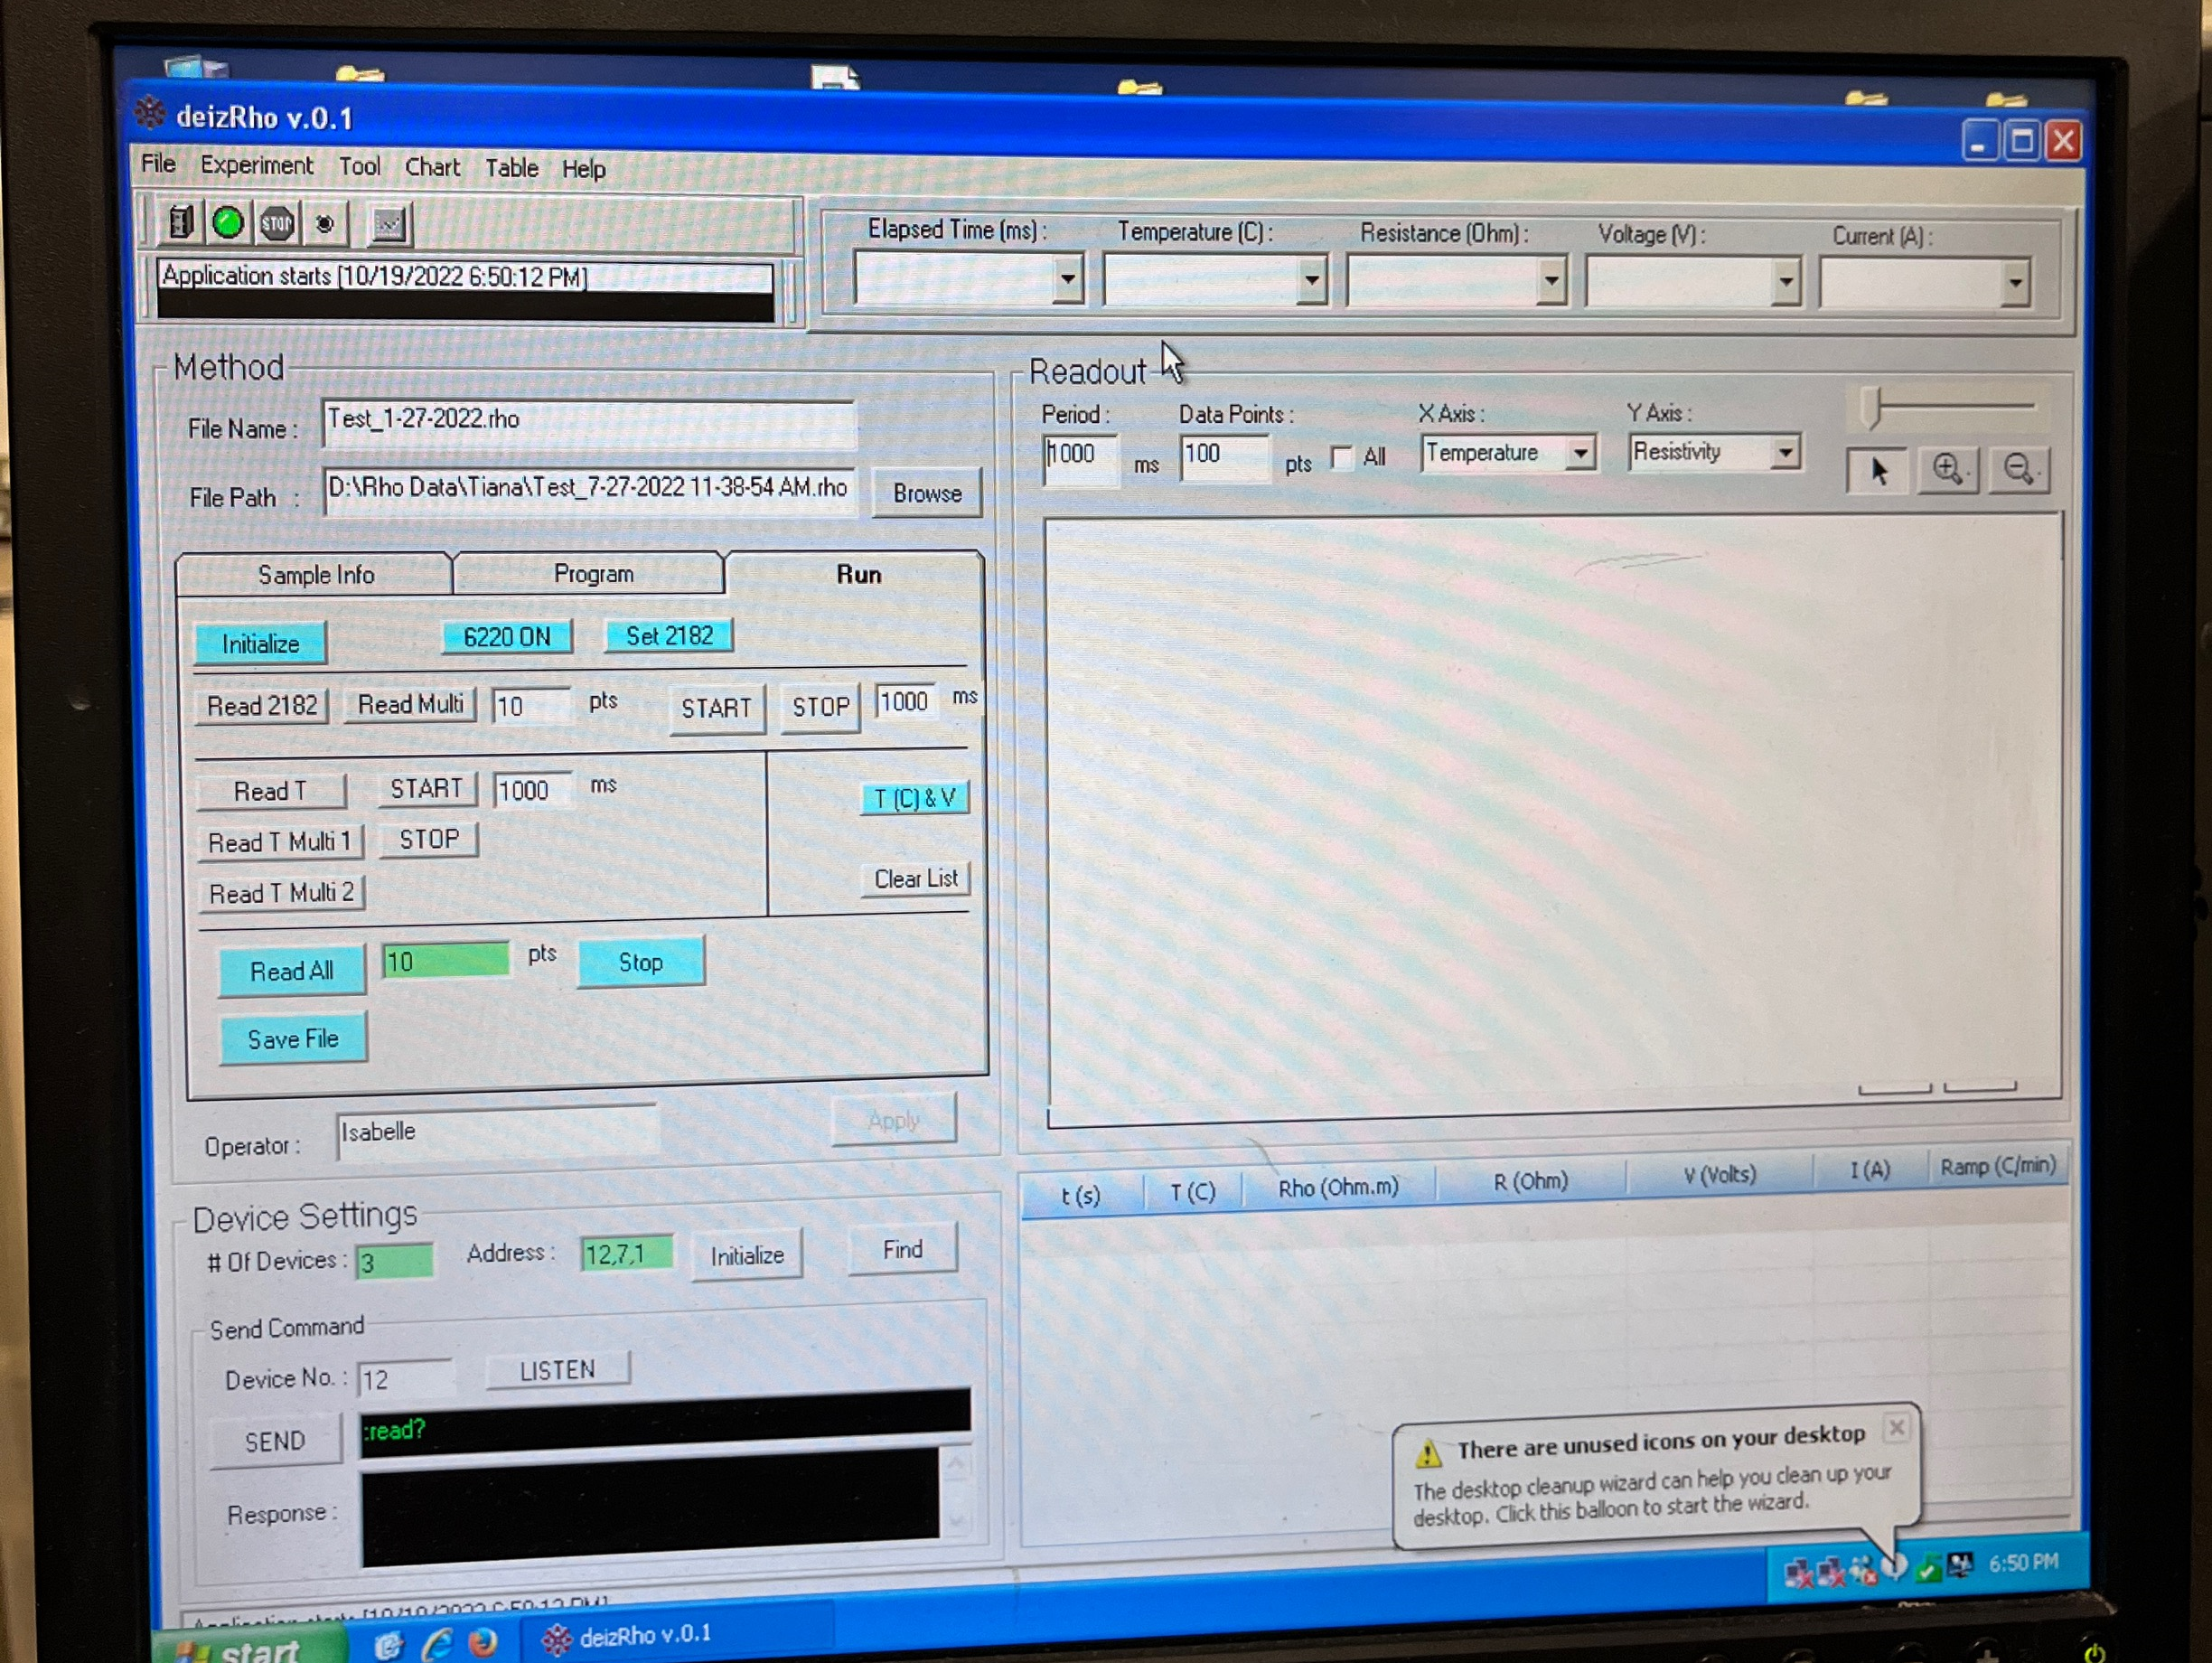
\includegraphics[scale=0.2]{app.png}}
\caption{Previous software user interface design}
\label{fig}
\end{figure}

\noindent The key elements of the existing implementation will also be included in our implementation. This is so that the application will be familiar to the user and as intuitive as possible. These elements are listed below:
\begin{itemize}
  \item Method Panel: controls which device to read data from (temperature or voltage), and which file to save the data in
  \item Device Settings Panel: used to send SCPI commands directly to a device
  \item Readout: includes graphical output and listed output of relevant values (current, voltage, resistance, etc.)
\end{itemize}

\noindent The primary differences between the existing implementation and our implementaion are the appearance of the GUI and the option of remote access. The existing implementation was developed for Windows XP whereas our implementation is developed for Windows 10, which gives it an updated look. One of the stretch goals for this project is to enable remote access to the application to be able to monitor and stop experiments remotely. The existing implementation does not have this functionality.\\


\section{Unit Testing}

\subsection{Calculation Module}
\begin{tabular}{ |p{1.5cm}||p{2.5cm}|p{3cm}|p{2cm}|p{2cm}|p{1.5cm}|}
  \hline
  \multicolumn{6}{|c|}{Unit Tests for Calculation Module} \\
  \hline
  Unit Test ID & Description & Input & Expected Output & Output & Result\\
  \hline
  UT-C1   & Testing the getResistance Method  &  From HardwareInput ADT: Voltage = 5, Current = 1 & 5.000 & 5.000 & PASS \\
  \hline
  UT-C1   & Testing the getResistance Method  &  From HardwareInput ADT: Voltage = 4, Current = 0.6 & 6.667 & 6.667 & PASS \\
  \hline
  UT-C2   & Testing the getResistance Method  &  From HardwareInput ADT: Voltage = -5, Current = 1 & Invalid & Invalid & PASS \\
  \hline
  UT-C2   & Testing the getResistance Method  &  From HardwareInput ADT: Voltage = -4, Current = 0.6 & Invalid & Invalid & PASS \\
  \hline
  UT-C3   & Testing the getResistivity Method  &  Resistance = 3, Area = 2.5, Length = 2 & 3.750 & 3.750 & PASS \\
  \hline
  UT-C3   & Testing the getResistivity Method  &  Resistance = 2, Area = 2.8, Length = 1 & 5.600 & 5.600 & PASS \\
 \end{tabular}

\section{Changes Due to Testing}

\noindent Based on the feedback from our Rev 0 Demo, we found that our application failed some requirements tests. The major failures were the lack of two main features: the graphical output (which still did not display real data as of Rev 0 Demo) and the ability to save output data to a chosen file. While we did not need to "test" our application to know this, we still consider these to be failed tests, as our application failed to meet requirements set out by the project supervisor. These two features have been implemented for the final demo. \\

\begin{tabular}{ |p{3cm}|p{5cm}|p{5cm}| }
  \hline
  \textbf{Test ID} & \textbf{Failure Observed} & \textbf{Change(s) Made} \\
  \hline 
  ST6 & Graph only displays dummy data & Bug with displaying real-time data was fixed \\ \hline
  ST7 & There is no method to output data to a file & File system browser and writing to output file was added \\
  \hline
 \end{tabular}


\section{Automated Testing}

\noindent We achieved automated unit testing through the use of the NUnit testing framework in Visual Studio. NUnit is one of the most popular test frameworks used for running tests on a .NET project.\\

\noindent NUnit tests are setup by first creating a new project file in Visual Studio and adding it to the solution file for your project (in our case, the application). In the new project file, a new class is created. Each unit test we want to carry out is written as a method of the test class. Since the project file for the test class is inlcuded in the same solution file as our application, we are able to call the test methods from our main application to run the tests.\\
		
\section{Trace to Requirements}
\begin{tabular}{ |p{3cm}||p{4cm}|p{4cm}|p{4cm}|p{4cm}| }
  \hline
  \multicolumn{4}{|c|}{Traceability Matrix to Non Functional Requirements} \\
  \hline
  Requirement Type & Requirement(SRS) & Test Requirement & Related Unit Tests \\
  \hline
  Non Functional   & NFR-U1  & NF-UT1 & U \\ \hline
  Non Functional   & NFR-U2  & NF-UT2 & U \\ \hline
  Non Functional   & NFR-U3  & NF-UT3 & U \\ \hline
  Non Functional   & NFR-U4  & NF-UT4 & U \\ \hline
  Non Functional   & NFR-U5  & NF-UT5 & U \\ \hline
  Non Functional   & NFR-U6  & NF-UT6 & U \\ \hline
  
 \end{tabular}

 \begin{tabular}{ |p{3cm}||p{4cm}|p{4cm}|p{4cm}|p{4cm}| }
  \hline
  \multicolumn{4}{|c|}{Traceability Matrix to Functional Requirements} \\
  \hline
  Requirement Type & Requirement(SRS) & Test Requirement & Related Unit Tests \\
  \hline
  Functional   & FR1  & FR-T1 & U \\ \hline
  Functional   & FR2  & FR-T2 & U \\ \hline
  Functional   & FR3  & FR-T3 & U \\ \hline
  Functional   & FR4  & FR-T4 & U \\ \hline
  Functional   & FR5  & FR-T5 & U \\ \hline
  Functional   & FR6  & FR-T6 & U \\ \hline
  
 \end{tabular}
		
\section{Trace to Modules}		

\bibliographystyle{plainnat}
\bibliography{../../refs/References}

\newpage{}
\section*{Appendix --- Reflection}

The information in this section will be used to evaluate the team members on the
graduate attribute of Lifelong Learning.  Please answer the following questions:

\begin{enumerate}
  \item In what ways was the Verification and Validation (VnV) Plan different
  from the activities that were actually conducted for VnV?  If there were
  differences, what changes required the modification in the plan?  Why did
  these changes occur?  Would you be able to anticipate these changes in future projects?  If there weren't any differences, how was your team able to clearly predict a feasible amount of effort and the right tasks needed to build the evidence that demonstrates the required quality?  (It is expected that most teams will have had to deviate from their original VnV Plan.)
\end{enumerate}

\indent There were several differences between what we had planned for VnV and what we ended up carrying out. When completing the initial revision of VnV plan, we had not yet completed the Design documents (MG, MIS, System Design) and so we did not have a plan for unit/module testing, only for system testing. Our initial VnV plan included three main sections: SRS Verification, Design Verification, and Implementation Verification.\\

\indent For SRS Verification, we planned to meet every two weeks to discuss potential updates to the SRS doc. While we continued to meet frequently (weekly or bi-weekly), our team focussed instead on the next deliverable rather than revisiting old documents during meetings. Because of this, our SRS was not continually being updated during the project. This change occurred mainly due to time constraints, as we faced some technical issues leading up to the first demo which took priority over other tasks. In hindsight, frequently revisiting and updating the SRS certainly would have created less work for us in the long run. For future projects, though we can't predict any exact technical issues that would set us back on time, we should be able to anticipate issues arising which cause delays. We should have a plan to stay on schedule despite such issues. \\

\indent  For Design Verification, we planned to use the MIS checklist to ensure that requirements in the SRS are met and hazards in the Hazard Analysis are covered. Our team followed the MIS checklist when testing. We also planned to use feedback from the course instructor, teaching assistants, classmates, and our project supervisor. There were not many changes made in this section of the plan, except that our team decided to focus primarily on feedback from Dr. Zurob, as he is the end-user of the application. \\

\indent For Implementation Verification, we planned to used GitHub issues and pull requests to maintain our code base. Any pull request made to the main branch requires at least two other team members to review and approve. We did not make any major changes to our Implementation Verification plan. 
\end{document}